\lettrine[lines=2,slope=0pt,nindent=4pt]{\textbf{T}}{o} determine the flow of a fluid, it is necessary to describe the kinematics of all its
material particles throughout time. To do so, one can adopt either an Euler description
of motion, in which a fluid particle is identified by its initial position, or a Lagrange
description of motion, in which a fluid particle is identified by its instantaneous position.
Both descriptions are totally equivalent, leading to different forms of the Navier-Stokes
equations that can be discretized on a stationary mesh grid (Euler) or a mesh grid that
follows the motion of the fluid particles (Lagrange). In both cases, the mesh nodes do not
account for the motion of the boundaries, which makes the numerical simulations of the
related Navier-Stokes equations delicate. To overcome this problem, several approaches,
such as the immersed boundary methods, or the Arbitrary Lagrangian-Eulerian
(ALE) method have been developed.\smallskip\newline

Here, we rely on the ALE method. In the ALE approach, the fluid flow is computed in
a domain that is deformed in order to follow the movement of the fluid-solid interface. It
provides a hybrid description not associated with the fluid particles and the laboratory
coordinates. We associate the description with a moving imaginary mesh that follows the
fluid domain. The motion of the ALE computational mesh is independent of the material
motion, the approach treats the mesh as a frame that moves with an arbitrary velocity.
In the Eulerian approach, this velocity is zero, whereas it is equal to the velocity
of the fluid particles in the Lagrangian approach. But in the ALE method, this velocity
is equal to neither zero nor the velocity of the fluid particles; it varies smoothly and
arbitrarily between both of them. This method is a Lagrangian description in zones and
directions near a solid interface and Eulerian elsewhere.\smallskip\newline

In that part, three cases used ALE method are detailed:\vspace*{0.5cm}\newline
\hspace*{0.5cm} $\bullet$ Single-phase flow around a vibrating cylindrical tube\vspace*{0.5cm}\newline
\hspace*{0.5cm} $\bullet$ Hydrodynamic interaction of two cylinders subjected to small oscillations\vspace*{0.5cm}\newline
\hspace*{0.5cm} $\bullet$ Vibrations of a cylinder in a square tube bundle immersed in a viscous fluid (DIVA experiments)\vspace*{2cm}\newline
\begin{center}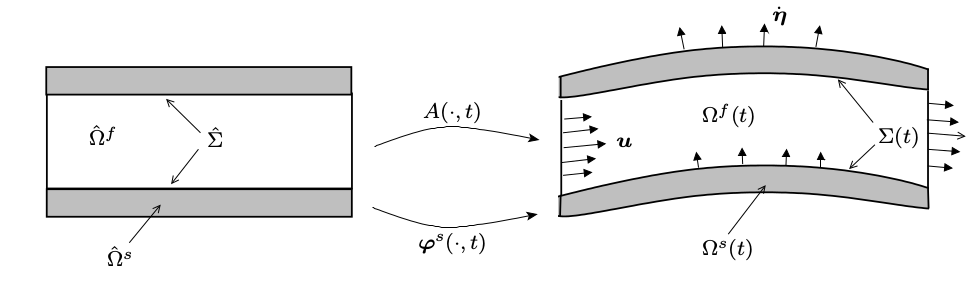
\includegraphics[width=14cm]{tools/MobileMesh.png}\end{center}
\texttt{\footnotesize{}extract from Donea J., Huerta A., Ponthot J. Ph. and Rodriguez-Ferran A., Encyclopedia of Computational Mechanic,
American Cancer Society, Arbitrary Lagrangian-Eulerian Methods, 2004}
